% Dokumentacja projektowa 
\newpage\section{Architektura systemu \NazwaSys}\label{sec:model}
% Odpowiedź na pytanie: Jak system działa?
\subsection{Schemat bazy danych} 
\begin{figure}[h!]
\centering
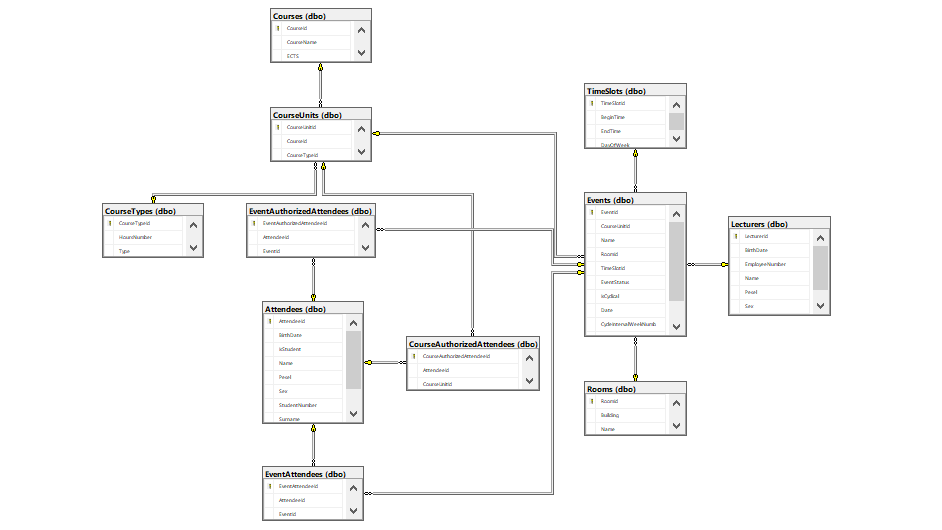
\includegraphics[width=16cm]{BD.png}
\caption{Schemat bazy danych}
\label{fig:schemat}
\end{figure}

\subsection{Moduł importu i eksportu danych}
Inferfejs administracyjny systemu podczas działania korzysta z interfejsu webowego stworzonego zgodnie z zasadami REST. Interfejs ten wykorzystuje notację JSON do serializacji zwracanych danych oraz protokół HTTP do komunikacji.

\subsection{Wnioski}
\begin{itemize}
    \item Wykorzystanie wzorca REST API oraz formatu danych JSON pozwala integrację systemu z innymi modułami stworzonymi na dowolnej platformie z wykorzystaniem dowolnego języka programowania wspierającego w.w. technologie.
\end{itemize}
